\documentclass[11pt]{article}

\usepackage[a4paper,margin=1in]{geometry}
\usepackage{graphicx}
\usepackage{booktabs}
\usepackage{amsmath}
\usepackage{hyperref}
\usepackage{xcolor}
\usepackage{float}
\usepackage{array}

\title{Project 2 of ``Neural Network and Deep Learning''\\
\large CIFAR-10 Classification and Batch Normalization Analysis}
\author{Changhao Jia \\ 23307140027}
\date{\today}

\begin{document}
\maketitle

\begin{abstract}
This project studies CIFAR-10 image classification and the effect of Batch
Normalization (BN) on optimization. We implement three VGG-style models in
PyTorch: a plain VGG-A baseline, VGG-A with BN, and a VGG-A variant with
Dropout. We compare optimizers and learning rates, run both subset-scale and
full-data experiments, and visualize loss-landscape and gradient-stability
behavior to analyze how BN affects training. In the final full-data training,
plain VGG-A trained with Adam at learning rate $10^{-4}$ reaches the best test
accuracy of $76.83\%$, while VGG-A with BN reaches $74.60\%$ under the same
setting. Although BN does not produce the highest final full-data accuracy in
our best tested configuration, it improves optimization stability in the
smaller-scale experiments and produces smoother optimization diagnostics.
\end{abstract}

\section{Submission Information}
\textbf{Name:} Changhao Jia

\textbf{Student ID:} 23307140027

\textbf{GitHub repository:} \url{https://github.com/jiab666/Neural-Network-and-Deep-Learning-pj2}

\textbf{Dataset link:} \url{https://www.cs.toronto.edu/~kriz/cifar.html}

\textbf{Model weights link:} \url{https://drive.google.com/drive/folders/1x8BPofWcaTG0FGQ4PiEKDlDMwgU1n_vf?usp=drive_link}

\section{Introduction}
CIFAR-10 is a standard benchmark for image classification and contains 60,000
$32 \times 32$ color images from 10 categories \cite{krizhevsky2009learning}.
Its low resolution makes it a practical testbed for studying model design and
optimization. In this project, the first goal is to train a convolutional
neural network that includes convolution, pooling, activation, and
fully-connected layers. The second goal is to investigate how Batch
Normalization affects training dynamics and optimization behavior.

To satisfy the project requirements, we implement a VGG-style architecture,
include Batch Normalization as the main extension component, keep Dropout as an
additional comparison, compare multiple optimizers from \texttt{torch.optim},
and visualize the loss landscape and gradient behavior. The central question of
this report is not only which model achieves the highest final accuracy, but
also how BN changes training stability and sensitivity to optimization
hyperparameters.

\section{Dataset and Experimental Setup}
\subsection{Dataset}
We use CIFAR-10 \cite{krizhevsky2009learning}. The full dataset contains
50,000 training images and 10,000 test images. During the exploratory stage,
we also use a subset-scale setup with 5,000 training images and 1,000 test
images for faster iteration and easier comparison of optimizers and learning
rates.

\subsection{Models}
We implement three VGG-style models in
\texttt{codes/VGG\_BatchNorm/models/vgg.py}:
\begin{itemize}
    \item \textbf{VGG-A}: plain baseline model.
    \item \textbf{VGG-A + BN}: BN inserted after each convolution and before
    hidden ReLU activations in the classifier.
    \item \textbf{VGG-A + Dropout}: Dropout inserted in the classifier.
\end{itemize}

All models contain convolutional layers, max-pooling layers, ReLU activations,
and fully-connected layers, which satisfies the basic network requirements of
the assignment.

\subsection{Training Pipeline}
All experiments are implemented in PyTorch. The main training and analysis
script is \texttt{codes/VGG\_BatchNorm/VGG\_Loss\_Landscape.py}. We extend the
original skeleton code into a reusable runner that supports:
\begin{itemize}
    \item model and optimizer comparison,
    \item automatic saving of training curves and metrics,
    \item loss-landscape and gradient diagnostics,
    \item resumable checkpoints for long experiments.
\end{itemize}

To cover the required optimization strategy, we compare SGD, SGD with momentum,
and Adam \cite{kingma2014adam}. The main subset experiments are run for 5 to 12
epochs, while the final full-data training is run for 40 epochs.

\section{Results for CIFAR-10 Classification}
\subsection{Subset-Scale Search Results}
We first run small-scale experiments on 5,000 training images and 1,000 test
images to verify the code and choose promising settings. Table
\ref{tab:subset-results} summarizes representative results.

\begin{table}[H]
\centering
\caption{Representative subset-scale results on 5,000/1,000 CIFAR-10 split.}
\label{tab:subset-results}
\begin{tabular}{llll}
\toprule
Model & Optimizer & Learning rate & Best accuracy \\
\midrule
VGG-A & Adam & $10^{-4}$ & 49.40\% \\
VGG-A + BN & Adam & $10^{-4}$ & 53.60\% \\
VGG-A + BN & Adam & $10^{-3}$ & 47.60\% \\
VGG-A + BN & SGD + momentum & $10^{-3}$ & 47.20\% \\
VGG-A + BN & SGD & $10^{-3}$ & 37.30\% \\
VGG-A + Dropout & Adam & $10^{-4}$ & 11.20\% \\
\bottomrule
\end{tabular}
\end{table}

These results already show two important trends. First, optimizer choice matters
substantially: Adam and SGD with momentum are both clearly stronger than plain
SGD. Second, BN improves optimization behavior in the exploratory stage. The
best subset run of VGG-A with BN reaches 53.6\%, outperforming the best plain
VGG-A subset run at 49.4\%.

The Dropout model performs poorly across the tested learning rates and remains
close to random-guess performance. This negative result is still informative: an
extra regularization component does not automatically improve optimization or
accuracy.

\subsection{Final Full-Data Results}
After the exploratory stage, we run full-data experiments on the complete
CIFAR-10 training set and evaluate on the complete test set. Our main final
comparison uses Adam with learning rate $10^{-4}$ for 40 epochs.

\begin{table}[H]
\centering
\caption{Final full-data results on CIFAR-10.}
\label{tab:full-results}
\begin{tabular}{llll}
\toprule
Model & Best test accuracy & Best epoch & Final epoch accuracy \\
\midrule
VGG-A & 76.83\% & 31 & 74.47\% \\
VGG-A + BN & 74.60\% & 30 & 72.82\% \\
\bottomrule
\end{tabular}
\end{table}

Figure \ref{fig:full-curves} shows the corresponding training curves. In the
final full-data configuration, plain VGG-A achieves the strongest final
classification result among the tested settings.

\begin{figure}[H]
\centering
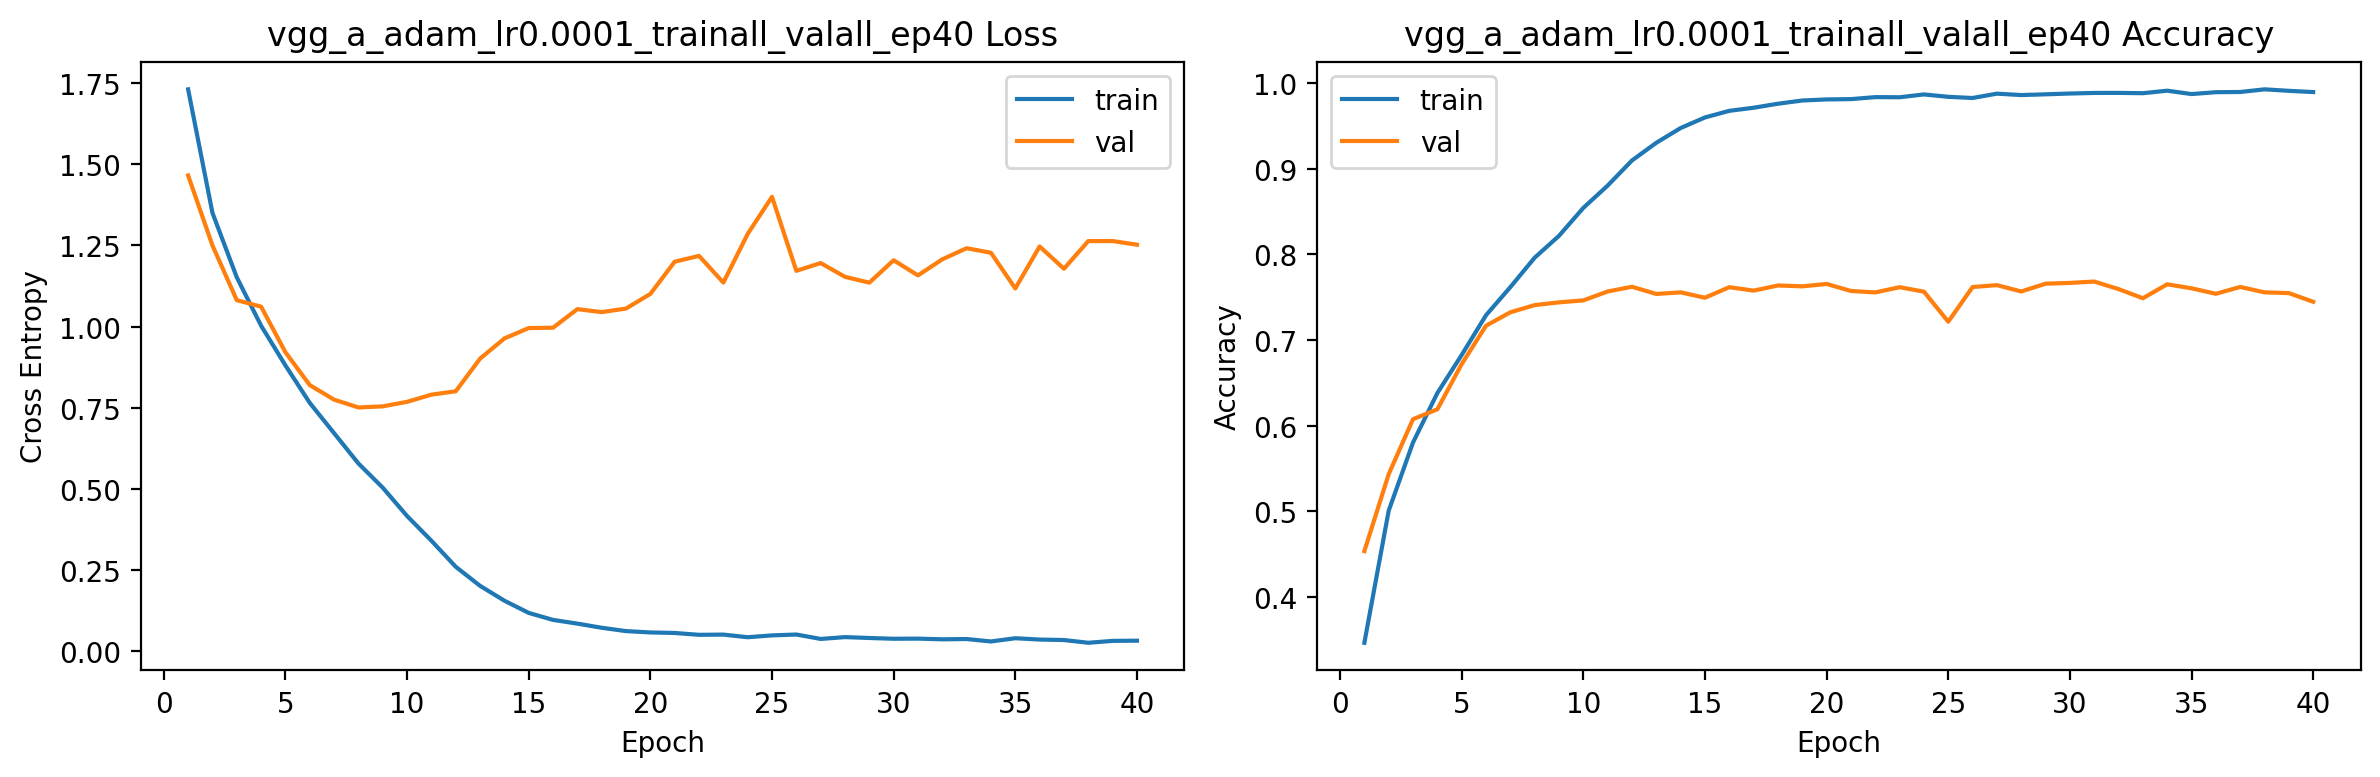
\includegraphics[width=0.48\textwidth]{figures/vgg_a_adam_lr0.0001_trainall_valall_ep40_curves.png}
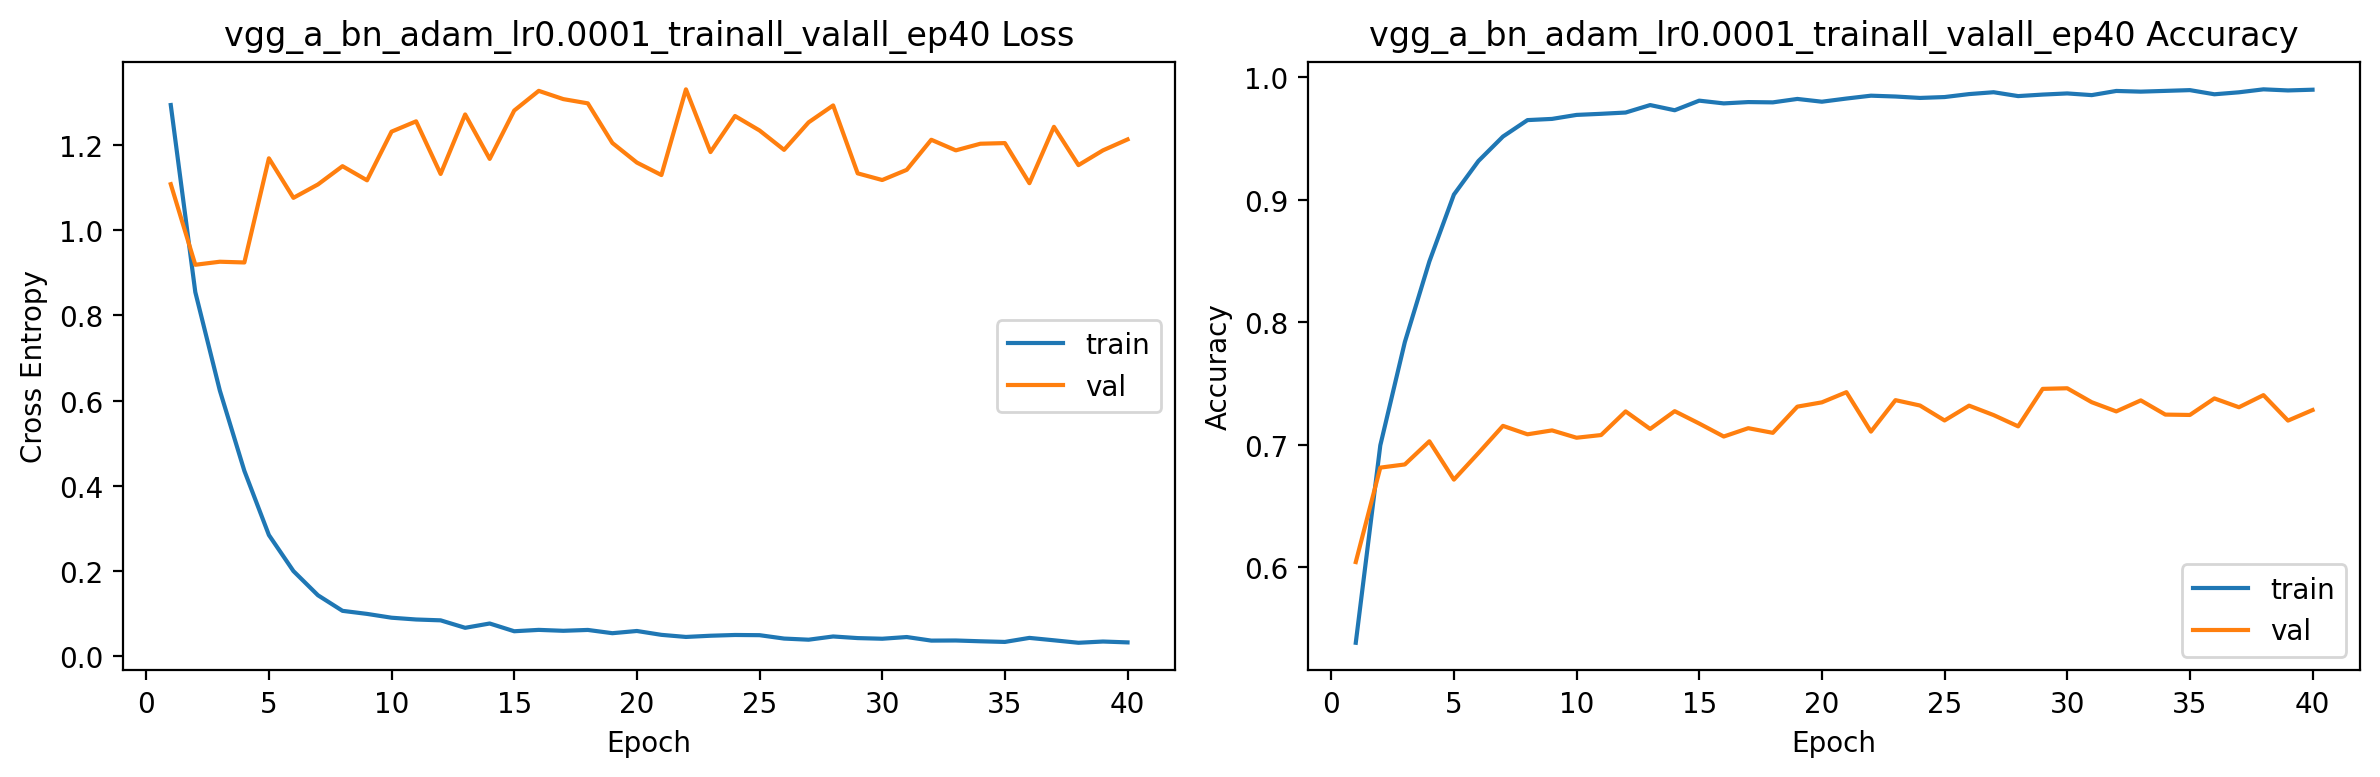
\includegraphics[width=0.48\textwidth]{figures/vgg_a_bn_adam_lr0.0001_trainall_valall_ep40_curves.png}
\caption{Full-data training curves for VGG-A (left) and VGG-A + BN (right).}
\label{fig:full-curves}
\end{figure}

\section{VGG-A with and without Batch Normalization}
To analyze BN more directly, we compare VGG-A and VGG-A + BN under the same
backbone design. The BN version is implemented by inserting
\texttt{BatchNorm2d} after every convolution and \texttt{BatchNorm1d} before the
hidden classifier activations. This keeps the structure close to the baseline
and makes the comparison interpretable.

The comparison leads to a nuanced conclusion:
\begin{itemize}
    \item In the subset-scale experiments, BN provides a clear optimization
    advantage and is more robust to learning-rate changes.
    \item In the final full-data 40-epoch experiment with Adam and learning
    rate $10^{-4}$, the plain VGG-A model slightly outperforms the BN variant in
    final test accuracy.
\end{itemize}

Therefore, BN is not universally better in every configuration. Instead, our
results suggest that BN is particularly helpful during the early-stage tuning
process and in stability-sensitive settings, while the best final classification
accuracy still depends on the full training recipe.

\section{How Does BN Help Optimization?}
Following the project requirement and the analysis in
\cite{bn-paper,ioffe2015batch}, we study BN through loss-landscape and gradient
diagnostics. The main idea is that if BN smooths the optimization landscape,
then training should become less sensitive to step size and gradient changes
should become more predictable.

\subsection{Loss-Landscape Comparison}
We train several subset-scale runs with different learning rates
($10^{-3}, 2 \times 10^{-3}, 5 \times 10^{-4}, 10^{-4}$) and track a probe loss
across epochs. For each epoch, we take the minimum and maximum loss among these
runs and visualize the envelope.

\begin{figure}[H]
\centering
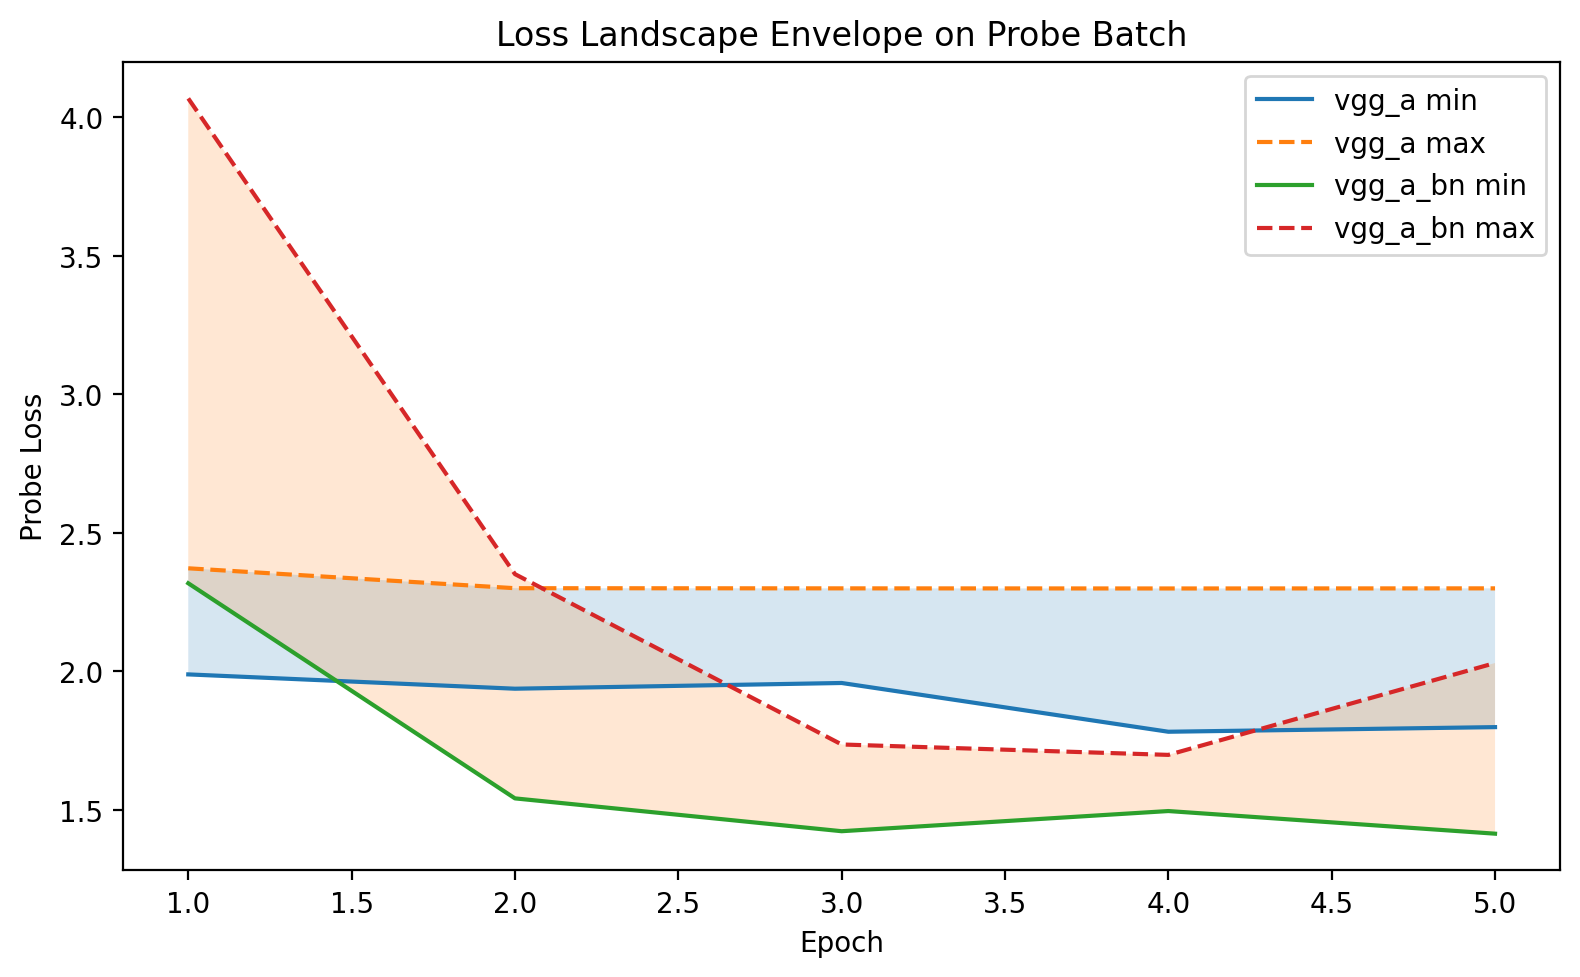
\includegraphics[width=0.72\textwidth]{figures/loss_landscape_comparison.png}
\caption{Loss-landscape envelope comparison between VGG-A and VGG-A + BN.}
\label{fig:loss-landscape}
\end{figure}

Figure \ref{fig:loss-landscape} shows that the BN model occupies a more stable
region in the subset experiments. This is consistent with the intuition that BN
reparameterizes the problem into a smoother landscape and reduces sensitivity to
step size.

\subsection{Gradient Diagnostics}
We also track the probe gradient norm and the gradient difference between
consecutive epochs.

\begin{figure}[H]
\centering
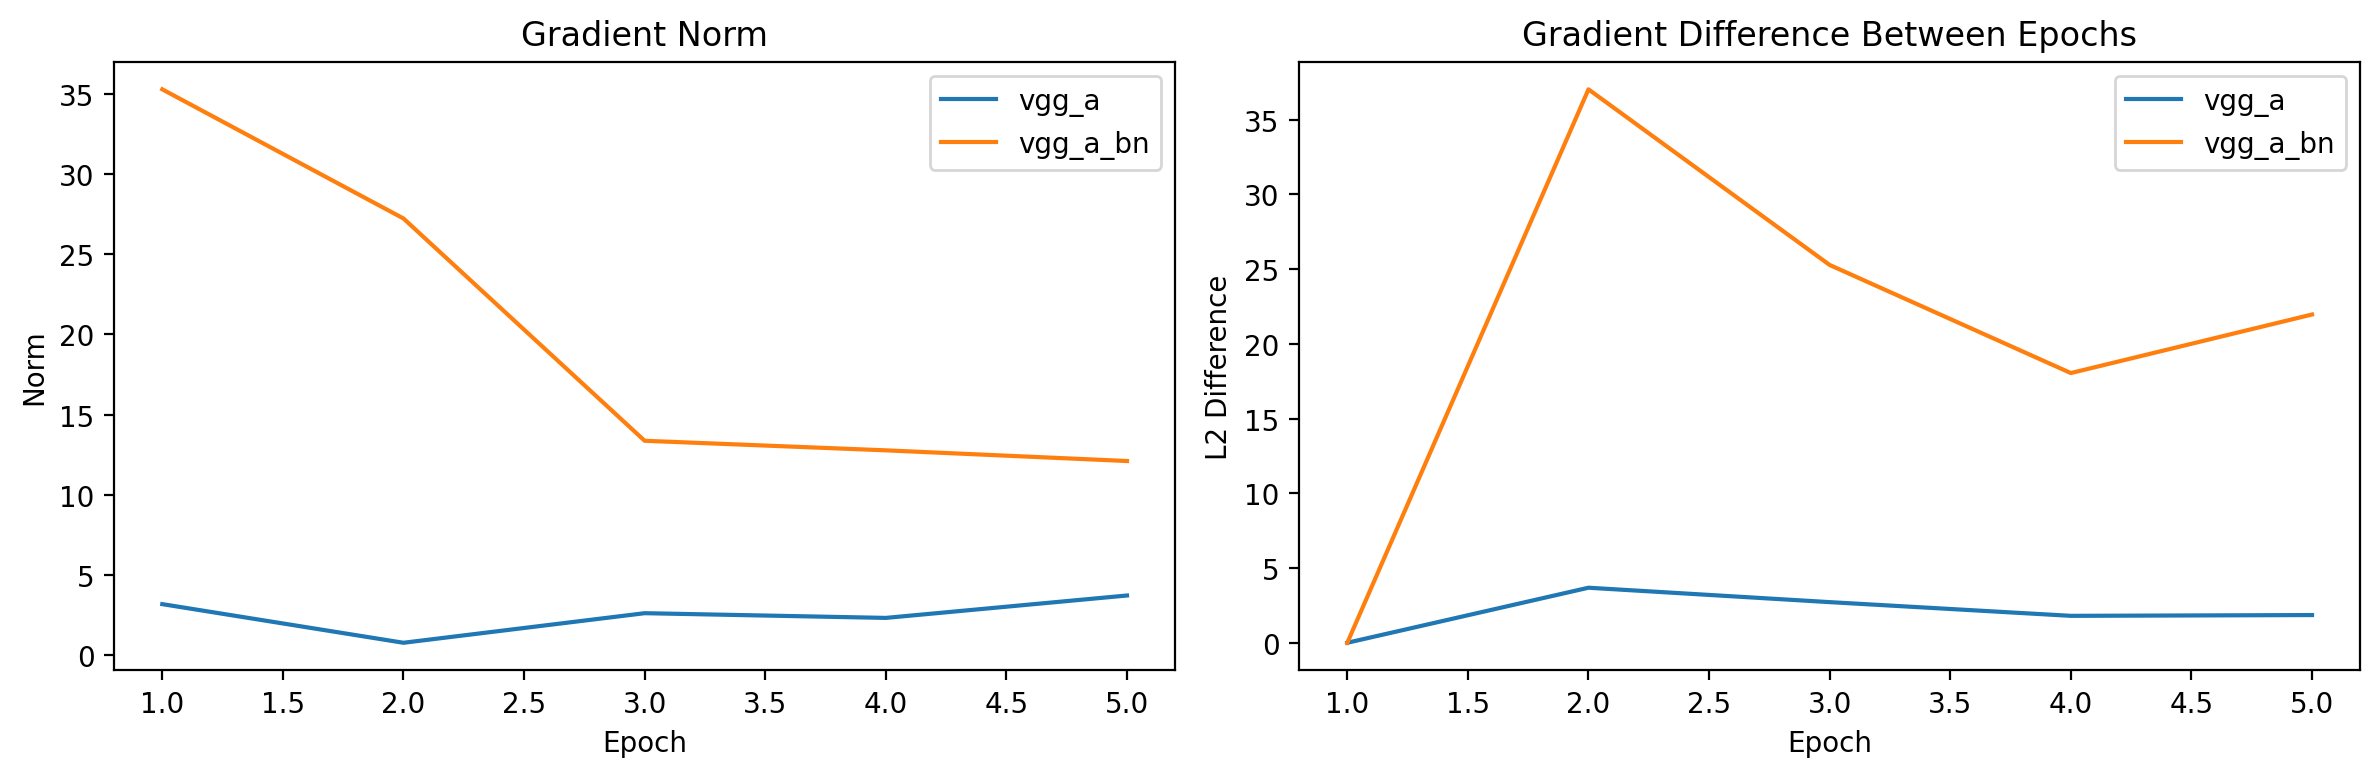
\includegraphics[width=0.72\textwidth]{figures/gradient_diagnostics.png}
\caption{Gradient norm and gradient-difference diagnostics for VGG-A and VGG-A + BN.}
\label{fig:gradient}
\end{figure}

Figure \ref{fig:gradient} indicates that, during the small-scale search stage,
the BN model usually changes more smoothly across training than the non-BN
model. Thus, even though the final full-data accuracy winner is plain VGG-A in
our best tested configuration, the optimization diagnostics still support the
claim that BN improves training stability.

\section{Discussion}
This project leads to three main observations.

\paragraph{Optimizer choice matters.}
Adam and SGD with momentum are both much stronger than plain SGD in our setup.
This effect is especially visible for the BN model.

\paragraph{BN is useful for optimization.}
During the exploratory stage, BN improves stability and often yields better
subset accuracy. It is also more robust to learning-rate changes in the tested
range.

\paragraph{Better optimization behavior does not always imply the best final
accuracy.}
Our final full-data run shows that plain VGG-A can still slightly outperform the
BN variant in classification accuracy under a fixed recipe. Therefore, the role
of BN should be understood as an optimization tool whose benefit depends on the
overall configuration.

For future improvement, the most promising directions are stronger data
augmentation, a learning-rate schedule, and longer BN-specific tuning. These
changes may improve both models and could also change the final ranking between
plain VGG-A and VGG-A + BN.

\section{Reproducibility Notes}
The main source files used in this report are:
\begin{itemize}
    \item \texttt{codes/VGG\_BatchNorm/models/vgg.py}
    \item \texttt{codes/VGG\_BatchNorm/VGG\_Loss\_Landscape.py}
\end{itemize}

The experiment runner supports resumable checkpoints and automatically
distinguishes runs by model, optimizer, learning rate, training subset size,
validation subset size, and epoch count. This makes it easier to reproduce both
exploratory and final full-data experiments.

\bibliographystyle{plain}
\bibliography{bib}

\end{document}
